\section{System Optimizations}

Our networks have tens of millions of parameters, and the training algorithm
takes tens of single-precision exaFLOPs to converge. Since our ability to
evaluate hypotheses about our data and models depends on the ability to train
models quickly, we built a highly optimized training system. This system has
two main components---a deep learning library written in \C++, along with a
high-performance linear algebra library written in both CUDA and \C++. Our
optimized software, running on dense compute nodes with 8 Titan X GPUs per
node, allows us to sustain 24 single-precision teraFLOP/second when training a
single model on one node. This is $45\%$ of the theoretical peak computational
throughput of each node. We also can scale to multiple nodes, as outlined in
the next subsection.

\subsection{Scalability and Data-Parallelism}

We use the standard technique of data-parallelism to train on multiple GPUs
using synchronous SGD. Our most common configuration uses a minibatch of $512$
on $8$ GPUs. Our training pipeline binds one process to each GPU. These
processes then exchange gradient matrices during the backpropagation by using
all-reduce, which exchanges a matrix between multiple processes and sums the
result so that at the end, each process has a copy of the sum of all matrices
from all processes. 

We find synchronous SGD useful because it is reproducible and deterministic. We
have found that the appearance of non-determinism in our system often signals a
serious bug, and so having reproducibility as a goal has greatly facilitates
debugging. In contrast, asynchronous methods such as asynchronous SGD with
parameter servers as found in Dean et al.~\cite{dean2012} typically do not
provide reproducibility and are therefore more difficult to debug. Synchronous
SGD is simple to understand and implement. It scales well as we add multiple
nodes to the training process.

\begin{figure}[h]
    \centering
    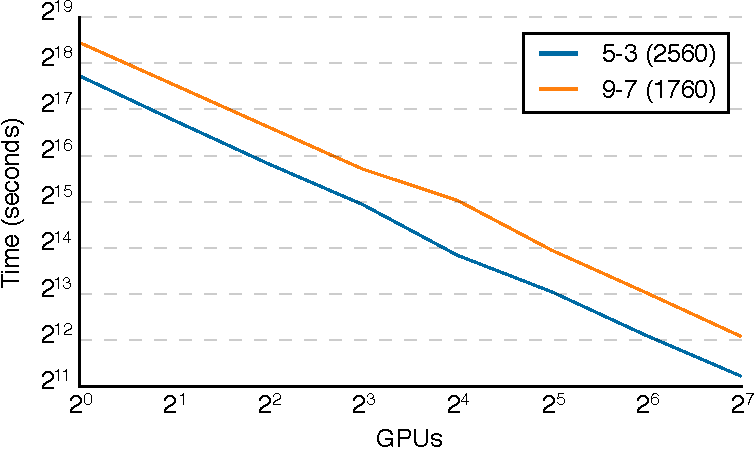
\includegraphics[width=0.6\textwidth]{deepspeech2/figures/weakscaling.pdf}
    \caption{Scaling comparison of two networks---a 5 layer model with 3
    recurrent layers containing 2560 hidden units in each layer and a 9 layer
    model with 7 recurrent layers containing 1760 hidden units in each layer.
    The times shown are to train 1 epoch.}
    \label{fig:deepspeech2:weakscaling}
\end{figure}

Figure~\ref{fig:deepspeech2:weakscaling} shows that time taken to train one
epoch halves as we double the number of GPUs that we train on, thus achieving
near-linear weak scaling. We keep the minibatch per GPU constant at 64 during
this experiment, effectively doubling the minibatch as we double the number of
GPUs. Although we have the ability to scale to large minibatches, we typically
use either 8 or 16 GPUs during training with a minibatch of 512 or 1024, in
order to converge to the best result.

Since all-reduce is critical to the scalability of our training, we wrote our
own implementation of the ring algorithm~\cite{patarasuk2009, thakur2005} for
higher performance and better stability. Our implementation avoids extraneous
copies between CPU and GPU, and is fundamental to our scalability. We configure
OpenMPI with the \emph{smcuda} transport that can send and receive buffers
residing in the memory of two different GPUs by using GPUDirect. When two GPUs
are in the same PCI root complex, this avoids any unnecessary copies to CPU
memory. This also takes advantage of tree-structured interconnects by running
multiple segments of the ring concurrently between neighboring devices. We
built our implementation using MPI send and receive, along with CUDA kernels
for the element-wise operations. 

Table~\ref{table:deepspeech2:allreduce} compares the performance of our all-reduce
implementation with that provided by OpenMPI version 1.8.5. We report the time
spent in all-reduce for a full training run that ran for one epoch on our
English dataset using a 5 layer, 3 recurrent layer architecture with $2560$
hidden units for all layers. In this table, we use a minibatch of 64 per GPU,
expanding the algorithmic minibatch as we scale to more GPUs. We see that our
implementation is considerably faster than OpenMPI's when the communication is
within a node (8 GPUs or less). As we increase the number of GPUs and increase
the amount of inter-node communication, the gap shrinks, although our
implementation is still 2-4X faster. 

\begin{table}
\centering
\begin{tabular}{r  r r r  r r r  r r r}
\toprule
GPU & \multicolumn{3}{c}{OpenMPI} & \multicolumn{3}{c}{Our} & \multicolumn{3}{c}{Performance} \\
    & \multicolumn{3}{c}{all-reduce} & \multicolumn{3}{c}{all-reduce} & \multicolumn{3}{c}{Gain}        \\
\midrule
4   & & 55359.1 & & & 2587.4 & & & 21.4 &  \\
8   & & 48881.6 & & & 2470.9 & & & 19.8 &  \\
16  & & 21562.6 & & & 1393.7 & & & 15.5 &  \\
32  & & 8191.8  & & & 1339.6 & & & 6.1  &  \\
64  & & 1395.2  & & & 611.0  & & & 2.3  &  \\
128 & & 1602.1  & & & 422.6  & & & 3.8  &  \\
\bottomrule
\end{tabular}
\caption{Comparison of two different all-reduce implementations. All times are
         in seconds. Performance gain is the ratio of OpenMPI all-reduce time to our
         all-reduce time.}
\label{table:deepspeech2:allreduce}
\end{table}

All of our training runs use either 8 or 16 GPUs, and in this regime, our
all-reduce implementation results in $2.5\times$ faster training for the full
training run, compared to using OpenMPI directly. Optimizing all-reduce has
thus resulted in important productivity benefits for our experiments, and has
made our simple synchronous SGD approach scalable.

\subsection{GPU implementation of CTC loss function}

Calculating the CTC loss function is more complicated than performing forward
and back propagation on our RNN architectures. Originally, we transferred
activations from the GPUs to the CPU, where we calculated the loss function
using an OpenMP parallelized implementation of CTC. However, this
implementation limited our scalability rather significantly, for two reasons.
Firstly, it became computationally more significant as we improved efficiency
and scalability of the RNN itself. Secondly, transferring large activation
matrices between CPU and GPU required us to spend interconnect bandwidth for
CTC, rather than on transferring gradient matrices to allow us to scale using
data parallelism to more processors.

To overcome this, we wrote a GPU implementation of the CTC loss function. Our
parallel implementation relies on a slight refactoring to simplify the
dependences in the CTC calculation, as well as the use of optimized parallel
sort implementations from ModernGPU~\cite{baxter2013}.

\begin{table}
\centering
\begin{tabular}{l  l  c  c  c}
\toprule
Language  & Architecture   & CPU CTC Time & GPU CTC Time  & Speedup  \\
\midrule
English   & 5-layer, 3 RNN & 5888.12      & 203.56        & 28.9     \\
Mandarin  & 5-layer, 3 RNN & 1688.01      & 135.05        & 12.5     \\
\bottomrule
\end{tabular}
\caption{Comparison of time spent in seconds in computing the CTC loss function
         and gradient in one epoch for two different implementations. Speedup is the
         ratio of CPU CTC time to GPU CTC time.}
\label{table:deepspeech2:gpucpuctc}
\end{table}

Table~\ref{table:deepspeech2:gpucpuctc} compares the performance of two CTC
implementations. The GPU implementation saves us 95 minutes per epoch in
English, and 25 minutes in Mandarin. This reduces overall training time by
10-20\%, which is also an important productivity benefit for our experiments.


\subsection{Memory allocation}

Our system makes frequent use of dynamic memory allocations to GPU and CPU
memory, mainly to store activation data for variable length utterances, and for
intermediate results. Individual allocations can be very large; over 1 GB for
the longest utterances.  For these very large allocations we found that CUDA's
memory allocator and even \texttt{std::malloc} introduced significant overhead
into our application---over a 2x slowdown from using \texttt{std::malloc} in
some cases. This is because both \texttt{cudaMalloc} and \texttt{std::malloc}
forward very large allocations to the operating system or GPU driver to update
the system page tables. This is a good optimization for systems running
multiple applications, all sharing memory resources, but editing page tables is
pure overhead for our system where nodes are dedicated entirely to running a
single model. To get around this limitation, we wrote our own memory allocator
for both CPU and GPU allocations. Our implementation follows the approach of
the last level shared allocator in jemalloc: all allocations are carved out of
contiguous memory blocks using the buddy algorithm~\cite{knowlton1965}. To
avoid fragmentation, we preallocate all of GPU memory at the start of training
and subdivide individual allocations from this block. Similarly, we set the CPU
memory block size that we forward to \texttt{mmap} to be substantially larger
than \texttt{std::malloc}, at 12GB.

Most of the memory required for training deep recurrent networks is used to
store activations through each layer for use by back propagation, not to store
the parameters of the network. For example, storing the weights for a 70M
parameter network with 9 layers requires approximately 280 MB of memory, but
storing the activations for a batch of 64, seven-second utterances requires 1.5
GB of memory. TitanX GPUs include 12GB of GDDR5 RAM, and sometimes very deep
networks can exceed the GPU memory capacity when processing long utterances.
This can happen unpredictably, especially when the distribution of utterance
lengths includes outliers, and it is desirable to avoid a catastrophic failure
when this occurs. When a requested memory allocation exceeds available GPU
memory, we allocate page-locked GPU-memory-mapped CPU memory using
\texttt{cudaMallocHost} instead. This memory can be accessed directly by the
GPU by forwarding individual memory transactions over PCIe at reduced
bandwidth, and it allows a model to continue to make progress even after
encountering an outlier.

The combination of fast memory allocation with a fallback mechanism that allows
us to slightly overflow available GPU memory in exceptional cases makes the
system significantly simpler, more robust, and more efficient.
